%% Nothing to modify here.
%% make sure to include this before anything else

\documentclass[10pt,aspectratio=169]{beamer}
\usetheme{metropolis}
\usenavigationsymbolstemplate{}
\usepackage{tgcursor}

% packages
\usepackage{color}
\usepackage{listings}

% color definitions
\definecolor{mygreen}{rgb}{0,0.6,0}
\definecolor{mygray}{rgb}{0.5,0.5,0.5}
\definecolor{mymauve}{rgb}{0.58,0,0.82}

% re-format the title frame page
\makeatletter
\def\supertitle#1{\gdef\@supertitle{#1}}%
%\setbeamertemplate{title page}
%{
%  \vbox{}
%  \vfill
%  \begin{centering}
%  \begin{beamercolorbox}[sep=8pt,center]{title}
%      \usebeamerfont{supertitle}\@supertitle
%   \end{beamercolorbox}
%    \begin{beamercolorbox}[sep=8pt,center]{title}
%      \usebeamerfont{title}\inserttitle\par%
%      \ifx\insertsubtitle\@empty%
%      \else%
%        \vskip0.25em%
%        {\usebeamerfont{subtitle}\usebeamercolor[fg]{subtitle}\insertsubtitle\par}%
%      \fi%
%    \end{beamercolorbox}%
%    \vskip1em\par
%    \begin{beamercolorbox}[sep=8pt,center]{author}
%      \usebeamerfont{author}\insertauthor
%    \end{beamercolorbox}
%    \begin{beamercolorbox}[sep=8pt,center]{institute}
%      \usebeamerfont{institute}\insertinstitute
%    \end{beamercolorbox}
%    \begin{beamercolorbox}[sep=8pt,center]{date}
%      \usebeamerfont{date}\insertdate
%    \end{beamercolorbox}\vskip0.5em
%    {\usebeamercolor[fg]{titlegraphic}\inserttitlegraphic\par}
%  \end{centering}
%  \vfill
%}
\makeatother

% insert frame number
\expandafter\def\expandafter\insertshorttitle\expandafter{%
      \insertshorttitle\hfill%
\insertframenumber\,/\,\inserttotalframenumber}

% preset-listing options
\lstset{
  backgroundcolor=\color{white},
  % choose the background color;
  % you must add \usepackage{color} or \usepackage{xcolor}
  basicstyle=\footnotesize,
  % the size of the fonts that are used for the code
  breakatwhitespace=false,
  % sets if automatic breaks should only happen at whitespace
  breaklines=true,                 % sets automatic line breaking
  captionpos=b,                    % sets the caption-position to bottom
  commentstyle=\color{mygreen},    % comment style
  % deletekeywords={...},
  % if you want to delete keywords from the given language
  extendedchars=true,
  % lets you use non-ASCII characters;
  % for 8-bits encodings only, does not work with UTF-8
  frame=single,                    % adds a frame around the code
  keepspaces=true,
  % keeps spaces in text,
  % useful for keeping indentation of code
  % (possibly needs columns=flexible)
  keywordstyle=\color{blue},       % keyword style
  % morekeywords={*,...},
  % if you want to add more keywords to the set
  numbers=left,
  % where to put the line-numbers; possible values are (none, left, right)
  numbersep=5pt,
  % how far the line-numbers are from the code
  numberstyle=\tiny\color{mygray},
  % the style that is used for the line-numbers
  rulecolor=\color{black},
  % if not set, the frame-color may be changed on line-breaks
  % within not-black text (e.g. comments (green here))
  stepnumber=1,
  % the step between two line-numbers.
  % If it's 1, each line will be numbered
  stringstyle=\color{mymauve},     % string literal style
  tabsize=4,                       % sets default tabsize to 4 spaces
  title=\lstname
  % show the filename of files included with \lstinputlisting;
  % also try caption instead of title
}

% macro for code inclusion
\newcommand{\includecode}[2][c]{
	\lstinputlisting[caption=#2, style=custom#1]{#2}
}
	% nothing to do here
\usepackage[english]{babel}

\usepackage[utf8]{inputenc}

\newcommand{\course}{
	C introduction
}

\author{
}

\lstset{
	language = C,
	showspaces = false,
	showtabs = false,
	showstringspaces = false,
	escapechar = @,
	belowskip=-1.5em
}

\def\ContinueLineNumber{\lstset{firstnumber=last}}
\def\StartLineAt#1{\lstset{firstnumber=#1}}
\let\numberLineAt\StartLineAt

\makeatletter
%\def\beamer@verbatimreadframe{%
%	\begingroup%
%	\let\do\beamer@makeinnocent\dospecials%
%	\count@=127%
%	\@whilenum\count@<255 \do{%
%		\advance\count@ by 1%
%		\catcode\count@=11%
%	}%
%	\beamer@makeinnocent\^^L% and whatever other special cases
%	\beamer@makeinnocent\^^I% <-- PATCH: allows tabs to be written to temp file
%	\endlinechar`\^^M \catcode`\^^M=12%
%	\@ifnextchar\bgroup{\afterassignment\beamer@specialprocessframefirstline\let\beamer@temp=}{\beamer@processframefirstline}}%
%\makeatother
 % TODO modify this if you have not already done so

% meta-information
\usepackage{tikz}
\usepackage{hyperref}
\hypersetup{
	colorlinks=true,
	linkcolor=darkgray,
	urlcolor=blue,
}
\usepackage{graphicx}

\newcommand{\topic}{
    Basic program structure
}

% nothing to do here
\title{\topic}
\supertitle{\course}
\date{}

% the actual document
\begin{document}

\maketitle

\begin{frame}{Contents}
	\tableofcontents
\end{frame}

\section{Setup}
\subsection{}

\begin{frame}{Getting started}
	The slides are at \href{https://fsr.github.io/c-lessons/materials.html}{fsr.github.io/c-lessons/materials.html}\\
	\bigskip
	There will be tasks! You can find them at \href{http://fsr.github.io/c-lessons/}{fsr.github.io/c-lessons}\\
	\bigskip
	If you have questions, use the auditorium group: \href{https://auditorium.inf.tu-dresden.de/de/groups/110804109}{https://auditorium.inf.tu-dresden.de/de/groups/110804109}\\
	\bigskip
	In case of big trouble, write an e-mail to your tutor.\\
\end{frame}

\begin{frame}{Programs for programming}
	For developing our own programs, we will use two kinds of software:\\
	\bigskip
	\textbf{Plain} text editors:
	\begin{itemize}
		\item vim (powerful, but needs getting used to)
		\item gedit (easy to use, comes with Gnome)
		\item Notepad(++) (for Windows users)
	\end{itemize}
	\bigskip
	Compilers:
	\begin{itemize}
		\item \textbf{gcc}
		\item clang
	\end{itemize}
\end{frame}

\begin{frame}[fragile]{gcc for Unix-based operating systems}
	Ubuntu / Debian:
	\begin{lstlisting}[numbers=none]
sudo apt install gcc
\end{lstlisting}
	\bigskip
	Arch Linux:
	\begin{lstlisting}[numbers=none]
sudo pacman -S gcc
\end{lstlisting}
	\bigskip
	Mac OS X:
	\begin{lstlisting}[numbers=none]
brew install gcc
\end{lstlisting}
	\bigskip
	\textellipsis\ and you're done ;-)
\end{frame}

\begin{frame}{gcc for Windows (using \textit{MinGW})}
	MinGW is a port of the gnu tools for Windows.\\
	\bigskip
	1. Retrieve mingw-get-setup.exe from \url{https://cloudstore.zih.tu-dresden.de/index.php/s/xs7qdJWpfo2wmcJ}
\end{frame}

\begin{frame}{gcc for Windows (using \textit{MinGW})}
	\centerline{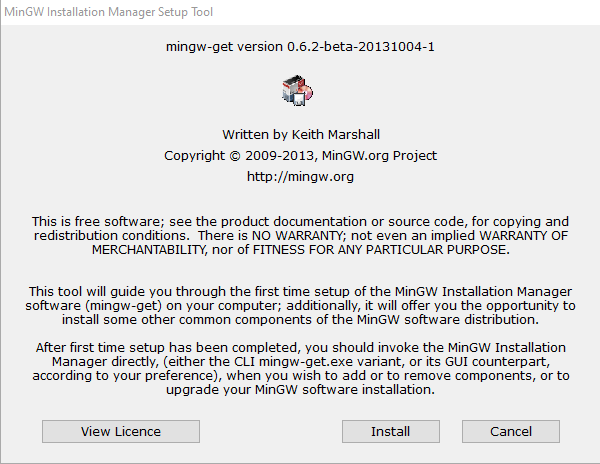
\includegraphics[scale=.45]{../img/install/mingw/setup.png}}
	\bigskip
	2. Install by executing mingw-get-setup.exe with admin rights
\end{frame}

\begin{frame}{gcc for Windows (using \textit{MinGW})}
	\centerline{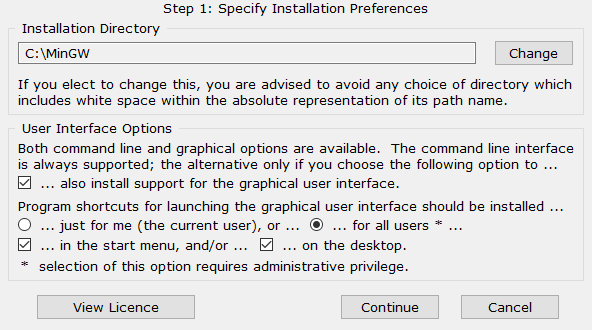
\includegraphics[scale=.5]{../img/install/mingw/settings.png}}
	\bigskip
	3. Select "for all users" and press "Continue"
\end{frame}

\begin{frame}{gcc for Windows (using \textit{MinGW})}
	\centerline{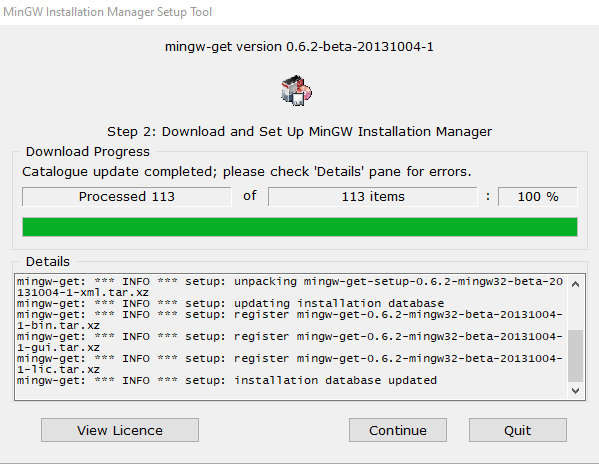
\includegraphics[scale=.45]{../img/install/mingw/finish.png}}
	\bigskip
	4. Press "Continue" when finished
\end{frame}

\begin{frame}{gcc for Windows (using \textit{MinGW})}
	\centerline{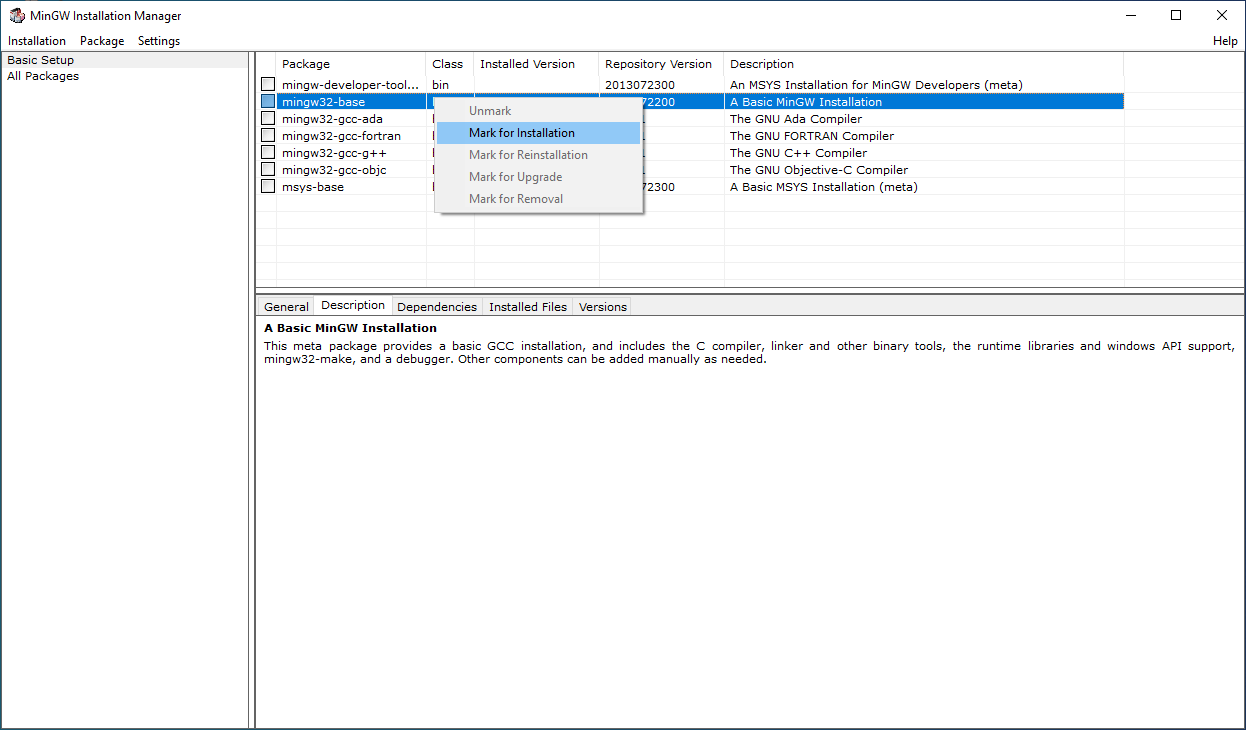
\includegraphics[scale=.3]{../img/install/mingw/mark.png}}
	\bigskip
	5. Mark the package "mingw32-base" for installation (right click)
\end{frame}

\begin{frame}{gcc for Windows (using \textit{MinGW})}
	\centerline{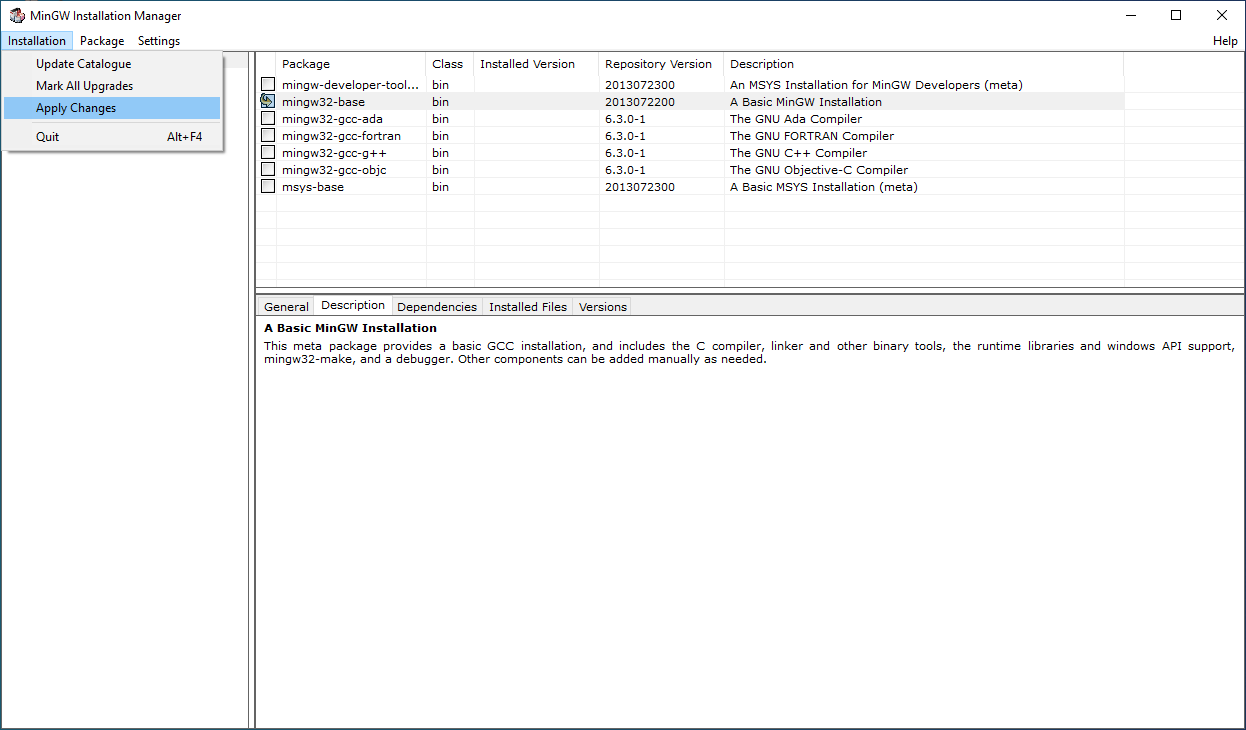
\includegraphics[scale=.3]{../img/install/mingw/apply.png}}
	\bigskip
	6. Select "Installation->Apply Changes"
\end{frame}

\begin{frame}{gcc for Windows (using \textit{MinGW})}
	\centerline{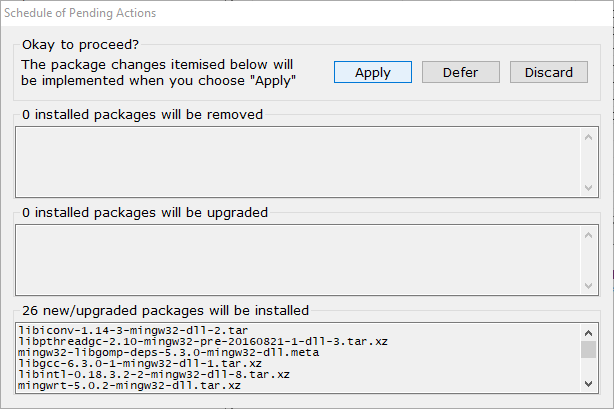
\includegraphics[scale=.5]{../img/install/mingw/confirm.png}}
	\bigskip
	7. Press "Apply" to proceed
\end{frame}

\begin{frame}{gcc for Windows (using \textit{MinGW})}
	\centerline{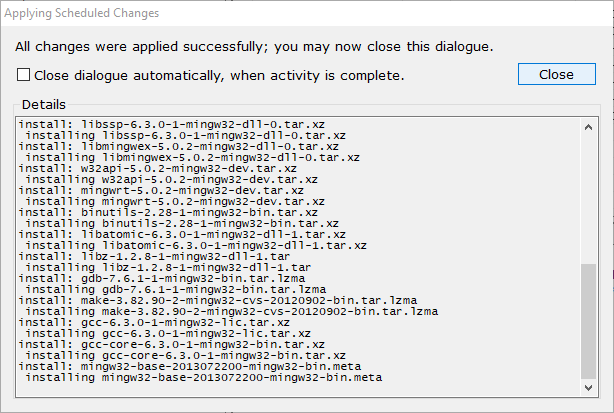
\includegraphics[scale=.5]{../img/install/mingw/close.png}}
	\bigskip
	8. Press "Close" when finished, you may close the Installation Manager now
\end{frame}

\begin{frame}{gcc for Windows (using \textit{MinGW})}
	\centerline{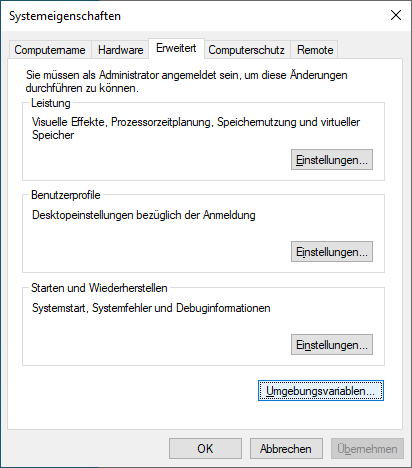
\includegraphics[scale=.45]{../img/install/path/properties.png}}
	\bigskip
	9. Now add gcc to PATH. Open "System Settings" and select "Environment Variables"
\end{frame}

\begin{frame}{gcc for Windows (using \textit{MinGW})}
	\centerline{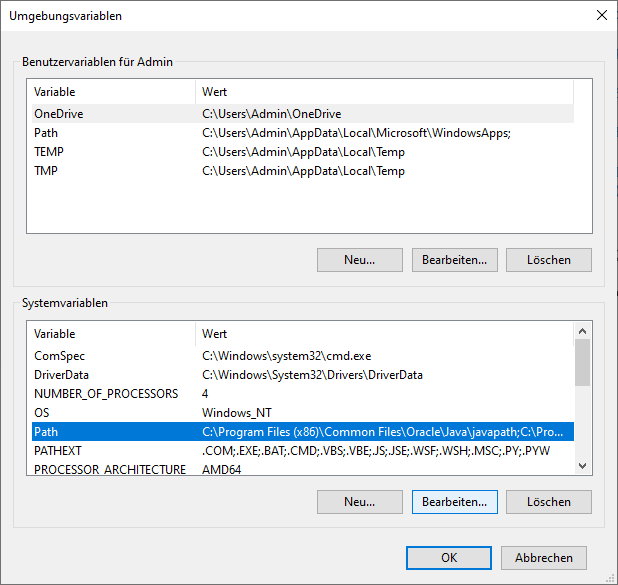
\includegraphics[scale=.35]{../img/install/path/edit.png}}
	\bigskip
	10. Edit "Path"
\end{frame}

\begin{frame}{gcc for Windows (using \textit{MinGW})}
	\centerline{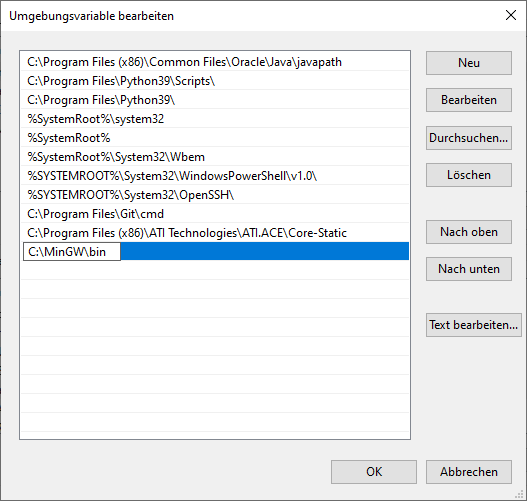
\includegraphics[scale=.4]{../img/install/path/path.png}}
	\bigskip
	11. Press "New" and add \path{C:\MinGW\bin} to path
\end{frame}

\begin{frame}{gcc for Windows (using \textit{MinGW})}
	12. Press "OK" and close "System Settings" \\
	\bigskip
	You can now test gcc with \textit{gcc --version}
\end{frame}

\section{Hello World!}
\subsection{}
\begin{frame}[fragile]{The first program}
	\begin{itemize}
		\item Create a new file named ``\textbf{main.c}''.
		\item Open it in your text editor of choice.
		\item Fill it as follows:
	\end{itemize}
	\begin{lstlisting}
#include <stdio.h>

int main(void)
{
	printf("Hello World!\n");
	/*
	 * Print "Hello World!" on the
	 * command line
	 */

	return 0;
}
\end{lstlisting}
\end{frame}
\begin{frame}[fragile]{From source to binary}
	\centering
	Source code\\\ \\
	$\Downarrow$\\\ \\
	\begin{lstlisting}[numbers=none]
gcc main.c
\end{lstlisting}
(Preprocessing, compiling, assembling, linking)
	\ \\\ \\
	$\Downarrow$\\\ \\
	Executable program\\\ \\
	\begin{columns}[T]
		\column{.35\textwidth}
		Linux/Mac OS X (\textbf{a.out})
		\begin{lstlisting}[numbers=none]
./a.out
\end{lstlisting}
		\column{.35\textwidth}
		Windows (\textbf{a.exe})
		\begin{lstlisting}[numbers=none]
.\a.exe
\end{lstlisting}
	\end{columns}
\end{frame}
\section{Program structure}
\subsection{}

\begin{frame}[fragile]{A basic program}
	\begin{columns}[T]
		\column{.6\textwidth}
		\begin{lstlisting}
#include <stdio.h>

int main(void)
{
	printf("Hello World!\n");
	
	/*
	 * Print "Hello World!" on the
	 * command line
	 */

	return 0;
}
\end{lstlisting}
		\column{.4\textwidth}
		
		\ \\$\left. \begin{array}{c}\\\end{array}\right\rbrace $ Preprocessor statements
		\ \\\ \\$\left. \begin{array}{c}\\\\\\\\\\\\\\\\\\\end{array}\right\rbrace $ Main function
	\end{columns}
\end{frame}
\begin{frame}[fragile]{Preprocessor statements}
	\begin{itemize}
		\item Processed before compilation
		\item Have their own language; start with a \textit{\#}
	\end{itemize}
	\begin{lstlisting}
#include <stdio.h>
\end{lstlisting}
	\begin{itemize}
		\item Includes the \textit{input/output header} from the \textbf{C standard library}
		\item Needed to use \textit{printf()}
	\end{itemize}\ \\ \ \\
	Preprocessor statements have way more use cases,\\
	but they form their own language which is very different from actual C.\\
	\bigskip
	In this course, we will use them for inclusions only.
\end{frame}
\begin{frame}[fragile]{The main function}
	\begin{itemize}
		\item Core function of every program
		\item Exists \textbf{exactly once} in every program
		\item Called on program start
	\end{itemize}
	\StartLineAt{3}
	\begin{lstlisting}
int main(void)
{
\end{lstlisting}
	\begin{itemize}
		\item As a function, \textit{main()} can take parameters and return a value
		\item Get used to \textit{void} and \textit{int}. They will be explained later
		\item '$\lbrace$' marks the start of the main function scope
	\end{itemize}
\end{frame}
\begin{frame}[fragile]{The main function scope}
	\begin{itemize}
		\item Contains program statements
		\item They are processed from top to bottom
	\end{itemize} \ \\
	\ \\
	\StartLineAt{9}
	\begin{lstlisting}
	return 0;
}
\end{lstlisting}
	\begin{itemize}
		\item Last statement; ends main function (and thus the whole program)
		\item \textit{0} tells the OS that everything went right
		\item '$\rbrace$' marks the end of the main function scope
	\end{itemize}
\end{frame}
\begin{frame}[fragile]{Statements}
	\begin{itemize}
		\item Instructions for the computer
		\item End with a \textit{;} (semicolon)
	\end{itemize}
	\StartLineAt{5}
	\begin{lstlisting}
	printf("Hello World!\n");
\end{lstlisting} \ \\ \ \\
	\begin{itemize}
		\item Here is the empty statement:
	\end{itemize}
	\begin{lstlisting}[numbers=none]
	;
\end{lstlisting}
	\begin{itemize}
		\item All statements are located in function blocks
	\end{itemize}
\end{frame}
\begin{frame}[fragile]{Comments}
	\begin{itemize}
		\item Information for you and others who use your code
		\item Cut out before compilation
	\end{itemize}
	Single-line comments:
	\StartLineAt{6}
	\begin{lstlisting}
	// Prints "Hello World!" on the command line
\end{lstlisting}
	Block comments (multi-line):
	\StartLineAt{6}
	\begin{lstlisting}
	/* Prints "Hello World!"
	   on the command line */
\end{lstlisting}
	Better style of block comments:
	\StartLineAt{6}
	\begin{lstlisting}
	/*
	 * Prints "Hello World!"
	 * on the command line
	 */
\end{lstlisting}
\end{frame}
\section{Style}
\subsection{}
\begin{frame}[fragile]{A few words on style}
	\begin{itemize}
		\item There can be multiple statements on one line
		\item Indentation is not necessary at all
		\item \textbf{But \textellipsis}
	\end{itemize}
	\ \\
	\begin{uncoverenv}<2->
	\begin{lstlisting}
#include <stdio.h>
int
main	(        void ){printf("Hello World!\n");
		// Prints
/*"Hello World!"			*/
		return 0;}
\end{lstlisting}
	\end{uncoverenv}
\end{frame}
\begin{frame}[fragile]{Write enjoyable code}
	\begin{itemize}
		\item Put each statement onto its own line
		\item Indent every statement in the main function by one \textit{tab}\\
		 or a fixed number of \textit{spaces}
		\item Decide on a commenting style and stick to it\\
		(\textit{/* .. */} recommended)
		\item Leave blank lines between different parts of the program
		\item Use \textit{spaces} and \textit{newlines} consistently
	\end{itemize}
	\begin{lstlisting}[showspaces=true,showtabs=true]
int main(void)
{
	printf("Hello World!");
	/* Prints "Hello World!" */

	return 0;
}
\end{lstlisting}
\end{frame}


% nothing to do from here on
\end{document}
